\section{}
在\textbf{图表示学习}阶段,我们首先收集并标注包含鸟类和其他物体(如水草、藻类等)的图片。使用目标检测算法(如 Faster R-CNN 或 YOLO)提取图片中的物体及其位置信息,将每个物体表示为图中的一个节点,物体之间的关系(如距离和角度)表示为边。接着,通过图神经网络(如 \textit{GCN})对图进行卷积操作,聚合节点及其邻居的信息,更新节点的特征表示。最后,将所有节点的特征汇聚为一个全局向量 \( H_{\text{global}} \),这个向量捕捉了图中所有节点和边的信息,为后续的方向和距离预测提供了基础。

\begin{figure}[h!]
\centering %图片居中
\subfloat[数据处理&特征提取]{
	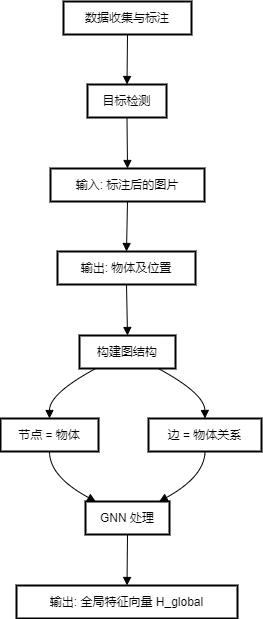
\includegraphics[width=0.35\textwidth]{figures/数据处理.drawio.png}
}
\end{figure}

\paragraph{}
说明:
数据收集与标注:获取带标注的鸟类图片数据。
目标检测:提取图片中的物体(如鸟类、背景元素)及其位置。
构建图结构:将物体作为节点,物体间关系(如空间距离)作为边。
GNN 处理:通过图神经网络生成全局特征向量。